\chapter{Analisi dei requisiti}
\label{cap:analisi-requisiti}

\intro{In questa sezione vengono analizzati i requisiti del progetto e ne viene data un’analisi ad alto livello, combinando
una visione concettuale con una visione pratica ed implementativa. Vengono inoltre descritti i casi d’uso e i requisiti
individuati, con l’obiettivo di fornire una visione generale del sistema e delle sue funzionalità, in modo semplice e
comprensibile.}\\

\section{Obiettivi dello stage}

Gli obiettivi fondamentali da raggiungere durante il periodo di tirocinio, stilati
in accordo con il tutor aziendale ed inseriti nel documento Piano di Lavoro, sono
identificati dalla seguente notazione:
\begin{itemize}
    \item \textbf{OO}: obiettivi obbligatori, vincolanti in quanto obiettivo primario richiesto dal committente;
    \item \textbf{OD}: obiettivi desiderabili, non vincolanti o strettamente necessari, ma dal riconoscibile valore aggiunto.
    \item \textbf{OZ}: obiettivi opzionali, non vincolanti e non necessari, ma che potrebbero essere implementati in un secondo momento.
\end{itemize}

Alle sigle precedentemente indicate seguirà un numero progressivo, identificando così
tutti gli obiettivi.\\
Essi sono i seguenti:
\begin{itemize}
    \item Obbligatori:
    \begin{itemize}
        \item \textbf{OO1}: acquisizione di competenze pratiche su Oribea/DialogSphere;
        \item \textbf{OO2}: connessione a database e gestione dati aziendali o pubblici;
        \item \textbf{OO3}: implementazione di un Task AI che genera un sistema di raccomandazioni e report automatico basato su analisi delle vendite;
        \item \textbf{OO4}: implementazione di un Task AI che permette di raccomandare prodotti ad un cliente in base ai suoi dati di vendita, e viceversa di raccomandare clienti ad un prodotto;
        \item \textbf{OO5}: generazione automatica di report con output coerente, chiaro e adattabile;
        \item \textbf{OO6}: testing e documentazione completa del prototipo.
    \end{itemize}
    \item Desiderabili:
    \begin{itemize}
        \item \textbf{OD1}: ottimizzazione del Task AI per performance e scalabilità;
        \item \textbf{OD2}: personalizzazione dinamica dei prompt per casi d’uso differenti;
        \item \textbf{OD3}: integrazione con strumenti di visualizzazione o interfacce utente.
    \end{itemize}
    \item Opzionali:
    \begin{itemize}
        \item \textbf{OZ1}: sviluppo di un chatbot o di una dashboard interattiva per l'interazione con il sistema di raccomandazioni e report;
        \item \textbf{OZ2}: sperimentazione di tecniche di Explainable AI (XAI) per la trasparenza dei risultati;
        \item \textbf{OZ3}: esportazione automatica dei report in PDF/HTML o invio via e-mail.
    \end{itemize}
\end{itemize}


\section{Casi d'uso}

Per lo studio dei casi di utilizzo delle due task sono stati creati dei diagrammi.\\
I diagrammi dei casi d'uso (in inglese \emph{Use Case Diagram}) sono diagrammi di tipo \gls{uml} dedicati alla descrizione delle funzioni o servizi offerti da un sistema, così come sono percepiti e utilizzati dagli attori che interagiscono col sistema stesso. Nel mio caso, l'unico attore che interagisce con le due task è l'utente semplice, che rappresenta un generico utente autenticato nella piattaforma Oribea.\\
Ciascun caso d’uso riporta gli attori coinvolti, le sue precondizioni, la sua descrizione, le sue postcondizioni ed eventuali sottocasi d’uso, inclusioni, specializzazioni e
scenari alternativi.\\
I casi d’uso che sono stati definiti sono i seguenti:

\begin{figure}[!h] 
    \centering 
    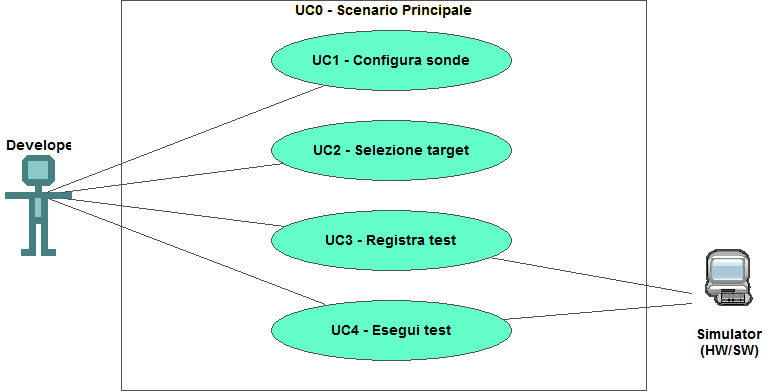
\includegraphics[width=0.9\columnwidth]{usecase/scenario-principale} 
    \caption{Use Case - UC0: Scenario principale}
\end{figure}

\begin{usecase}{0}{Scenario principale}
\usecaseactors{Sviluppatore applicativi}
\usecasepre{Lo sviluppatore è entrato nel plug-in di simulazione all'interno dell'IDE}
\usecasedesc{La finestra di simulazione mette a disposizione i comandi per configurare, registrare o eseguire un test}
\usecasepost{Il sistema è pronto per permettere una nuova interazione}
\label{uc:scenario-principale}
\end{usecase}

\section{Tracciamento dei requisiti}

Da un'attenta analisi dei requisiti e degli use case effettuata sul progetto è stata stilata la tabella che traccia i requisiti in rapporto agli use case.\\
Sono stati individuati diversi tipi di requisiti e si è quindi fatto utilizzo di un codice identificativo per distinguerli.\\
Il codice dei requisiti è così strutturato R(F/Q/V)(N/D/O) dove:
\begin{enumerate}
	\item[R =] requisito
    \item[F =] funzionale
    \item[Q =] qualitativo
    \item[V =] di vincolo
    \item[N =] obbligatorio (necessario)
    \item[D =] desiderabile
    \item[Z =] opzionale
\end{enumerate}
Nelle tabelle \ref{tab:requisiti-funzionali}, \ref{tab:requisiti-qualitativi} e \ref{tab:requisiti-vincolo} sono riassunti i requisiti e il loro tracciamento con gli use case delineati in fase di analisi.

\newpage

\begin{table}%
\caption{Tabella del tracciamento dei requisti funzionali}
\label{tab:requisiti-funzionali}
\begin{tabularx}{\textwidth}{lXl}
\hline\hline
\textbf{Requisito} & \textbf{Descrizione} & \textbf{Use Case}\\
\hline
RFN-1     & L'interfaccia permette di configurare il tipo di sonde del test & UC1 \\
\hline
\end{tabularx}
\end{table}%

\begin{table}%
\caption{Tabella del tracciamento dei requisiti qualitativi}
\label{tab:requisiti-qualitativi}
\begin{tabularx}{\textwidth}{lXl}
\hline\hline
\textbf{Requisito} & \textbf{Descrizione} & \textbf{Use Case}\\
\hline
RQD-1    & Le prestazioni del simulatore hardware deve garantire la giusta esecuzione dei test e non la generazione di falsi negativi & - \\
\hline
\end{tabularx}
\end{table}%

\begin{table}%
\caption{Tabella del tracciamento dei requisiti di vincolo}
\label{tab:requisiti-vincolo}
\begin{tabularx}{\textwidth}{lXl}
\hline\hline
\textbf{Requisito} & \textbf{Descrizione} & \textbf{Use Case}\\
\hline
RVO-1    & La libreria per l'esecuzione dei test automatici deve essere riutilizzabile & - \\
\hline
\end{tabularx}
\end{table}%
